%--------------------------------------------------------------------------------------------------
\chapter{Einbinden der Komponenten in das Projekt und Validierung der Anforderungen}\label{cha:ValidierungDesKonzepts}
In diesem Kapitel wird in den Unterkapiteln \ref{sec:MenschmodellEinbinden} und \ref{sec:ObjekteEinbinden} zunächst die Vorgehensweise für das Einbinden des Menschmodells und der Interaktionsschnittstelle in ein neues Projekt und das Einfügen neuer Objekte in der Umgebung erklärt. Daraufhin wird in den Unterkapiteln \ref{sec:ValidMensch} und \ref{sec:ValidInteraktion} erläutert, warum die in Kapitel \ref{sec:AnforderungenKonzept} gestellten Anforderungen an das Menschmodell und an die Interaktionsschnittstelle erfüllt werden.

%--------------------------------------------------------------------------------------------------
\section{Einbinden der Komponenten in ein neues Projekt}\label{sec:MenschmodellEinbinden}
Mit Hilfe der in diesem Abschnitt vorgestellten drei Schritte, soll das Einbinden des Menschmodells und der Interaktionsschnittstelle in ein beliebiges Projekt einfach gestaltet werden. Dabei sind die folgenden drei Schritte zu befolgen: Vorbereitung der Entwicklungsumgebung, Einfügen der Vorlagen in das neue Projekt und Einfügen in die Szene.

\paragraph{1. Vorbereitung der Entwicklungsumgebung}	
\noindent Im ersten Schritt muss die Entwicklungsumgebung vorbereitet werden. Dafür muss zunächst, mit Hilfe der in Kapitel \ref{sec:Software} erläuterten Programme VIVE Wireless und SteamVR, eine Verbindung mit der VR Hardware ermöglicht werden. Es ist zu empfehlen, die aktuellsten Versionen dieser Programme zu installieren. Des Weiteren muss die Unity Engine als Entwicklungsumgebung installiert werden. Dabei ist zu beachten, dass diese Arbeit, wie bereits in Kapitel \ref{sec:UnitEngine} erwähnt, mit Hilfe der Version 2019.2.19f1 von Unity entwickelt wurde. Daher empfiehlt es sich in Zukunft, sofern möglich, die gleiche Version zu verwenden. Schließlich müssen noch die in Kapitel \ref{sec:UnitEngine} erläuterten Plugins SteamVR und Final IK aus dem Asset Store heruntergeladen und in dem neuen Projekt importiert werden.

\paragraph{2. Einfügen der Vorlagen in das neue Projekt}
\noindent Im zweiten Schritt müssen die Vorlagen des Menschmodells und der Interaktionsschnittstelle in das neue Projekt eingefügt werden. Es ist ausreichend, die in Kapitel \ref{fig:UnityOverview} dargestellten Ordner 'Prefab', 'Scenes' und 'Scripts' zu kopieren und in das Verzeichnis des neuen Projekts einzufügen. Dabei ist anzumerken, dass ein Prefab in Unity eine Objektvorlage darstellt, die beliebig oft instanziiert werden kann. Daher befinden sich im Ordner 'Prefab' sämtliche Objektvorlagen des Projekts. In dem Ordner 'Scenes' befinden sich drei Demo-Szenen, unter anderem auch die in Abbildung \ref{fig:UnityOverview} dargestellte Szene und in dem Ordner 'Scripts' befinden sich sämtliche Skripte des Projekts. Eine genauere Erläuterung der Ordnerstruktur der zu kopierenden Verzeichnisse folgt im weiteren Verlauf dieses Kapitels.

\paragraph{3. Einfügen der Prefabs in die Szene}	
\noindent Im letzten Schritt muss lediglich das gewünschte Prefab in die neue Szene eingefügt werden. Dabei steht dem Entwickler frei, ob das Menschmodell ('Human'), die Interaktionsschnittstelle ('InteractionEventSystemAndScripts') oder beides zusammen ('Human+Interaction') in die neue Szene eingebunden werden soll. Für die Nutzung des Menschmodells, ohne die Interaktionsschnittstelle, muss lediglich das Prefab 'Human' aus dem gleichnamigen Ordner 'Human' (Vgl. Abbildung \ref{fig:Ordnerstruktur}) per Drag and Drop in der Szene eingefügt werden. Wenn jedoch die Interaktionsschnittstelle, ohne das Menschmodell, verwendet werden soll, muss neben dem Prefab der Interaktionsschnittstelle 'InteractionEventSystemAndScripts' aus dem Ordner 'InteractionPrefabs' (Vgl. Abbildung \ref{fig:Ordnerstruktur}), noch das Prefab des SteamVR CameraRigs aus dem Ordner 'Interaction Prefabs' (Vgl. Abbildung \ref{fig:Ordnerstruktur}), in der Szene eingefügt werden. Falls jedoch das Menschmodell, in Kombination mit der Interaktionsschnittstelle, verwendet werden soll, ist es ausreichend, wie in Abbildung \ref{fig:UnityOverview} dargestellt, lediglich das Prefab 'Human+Interaction' aus dem Ordner 'Prefab' (Vgl. Abbildung \ref{fig:Ordnerstruktur}) in der Szene zu platzieren.

\section{Hinzufügen neuer Objekte in der Umgebung}\label{sec:ObjekteEinbinden}
Genauso wie das Menschmodell inklusive der Interaktionsschnittstelle, können beliebige Objekte ohne großen Aufwand in die Umgebung des vorhandenen oder neuen Projekts integriert und für die Interaktionsschnittstelle einsatzfähig gemacht werden. Dabei sind die folgenden drei Schritte zu befolgen: Einfügen in die Ordnerstruktur des Projekts, Einsatzfähig für die Interaktionsschnittstelle machen und (optional) Einbinden in das vorhandene Menü.

\paragraph{1. Einfügen in die Ordnerstruktur des Projekts}
\noindent Bevor erklärt wird, wie genau neue Objekte in das Projekt und schließlich in die Szene eingefügt werden sollen, gibt es zunächst eine Einführung in den Aufbau der Ordnerstruktur des Projekts. Aufgrund dessen sind in Abbildung \ref{fig:Ordnerstruktur} die wichtigsten Ordner des Projekts ('Prefab', 'Scenes' und 'Scripts'), inklusive ausgewählter Unterordner, abgebildet. Es ist anzumerken, dass Ordner durch Rechtecke und Objekte durch Ovale abgebildet werden. Des Weiteren werden mit Hilfe von Pfeilen die zugehörigen Unterordner der einzelnen Ordner dargestellt.
\begin{figure}[h]
	\centering
	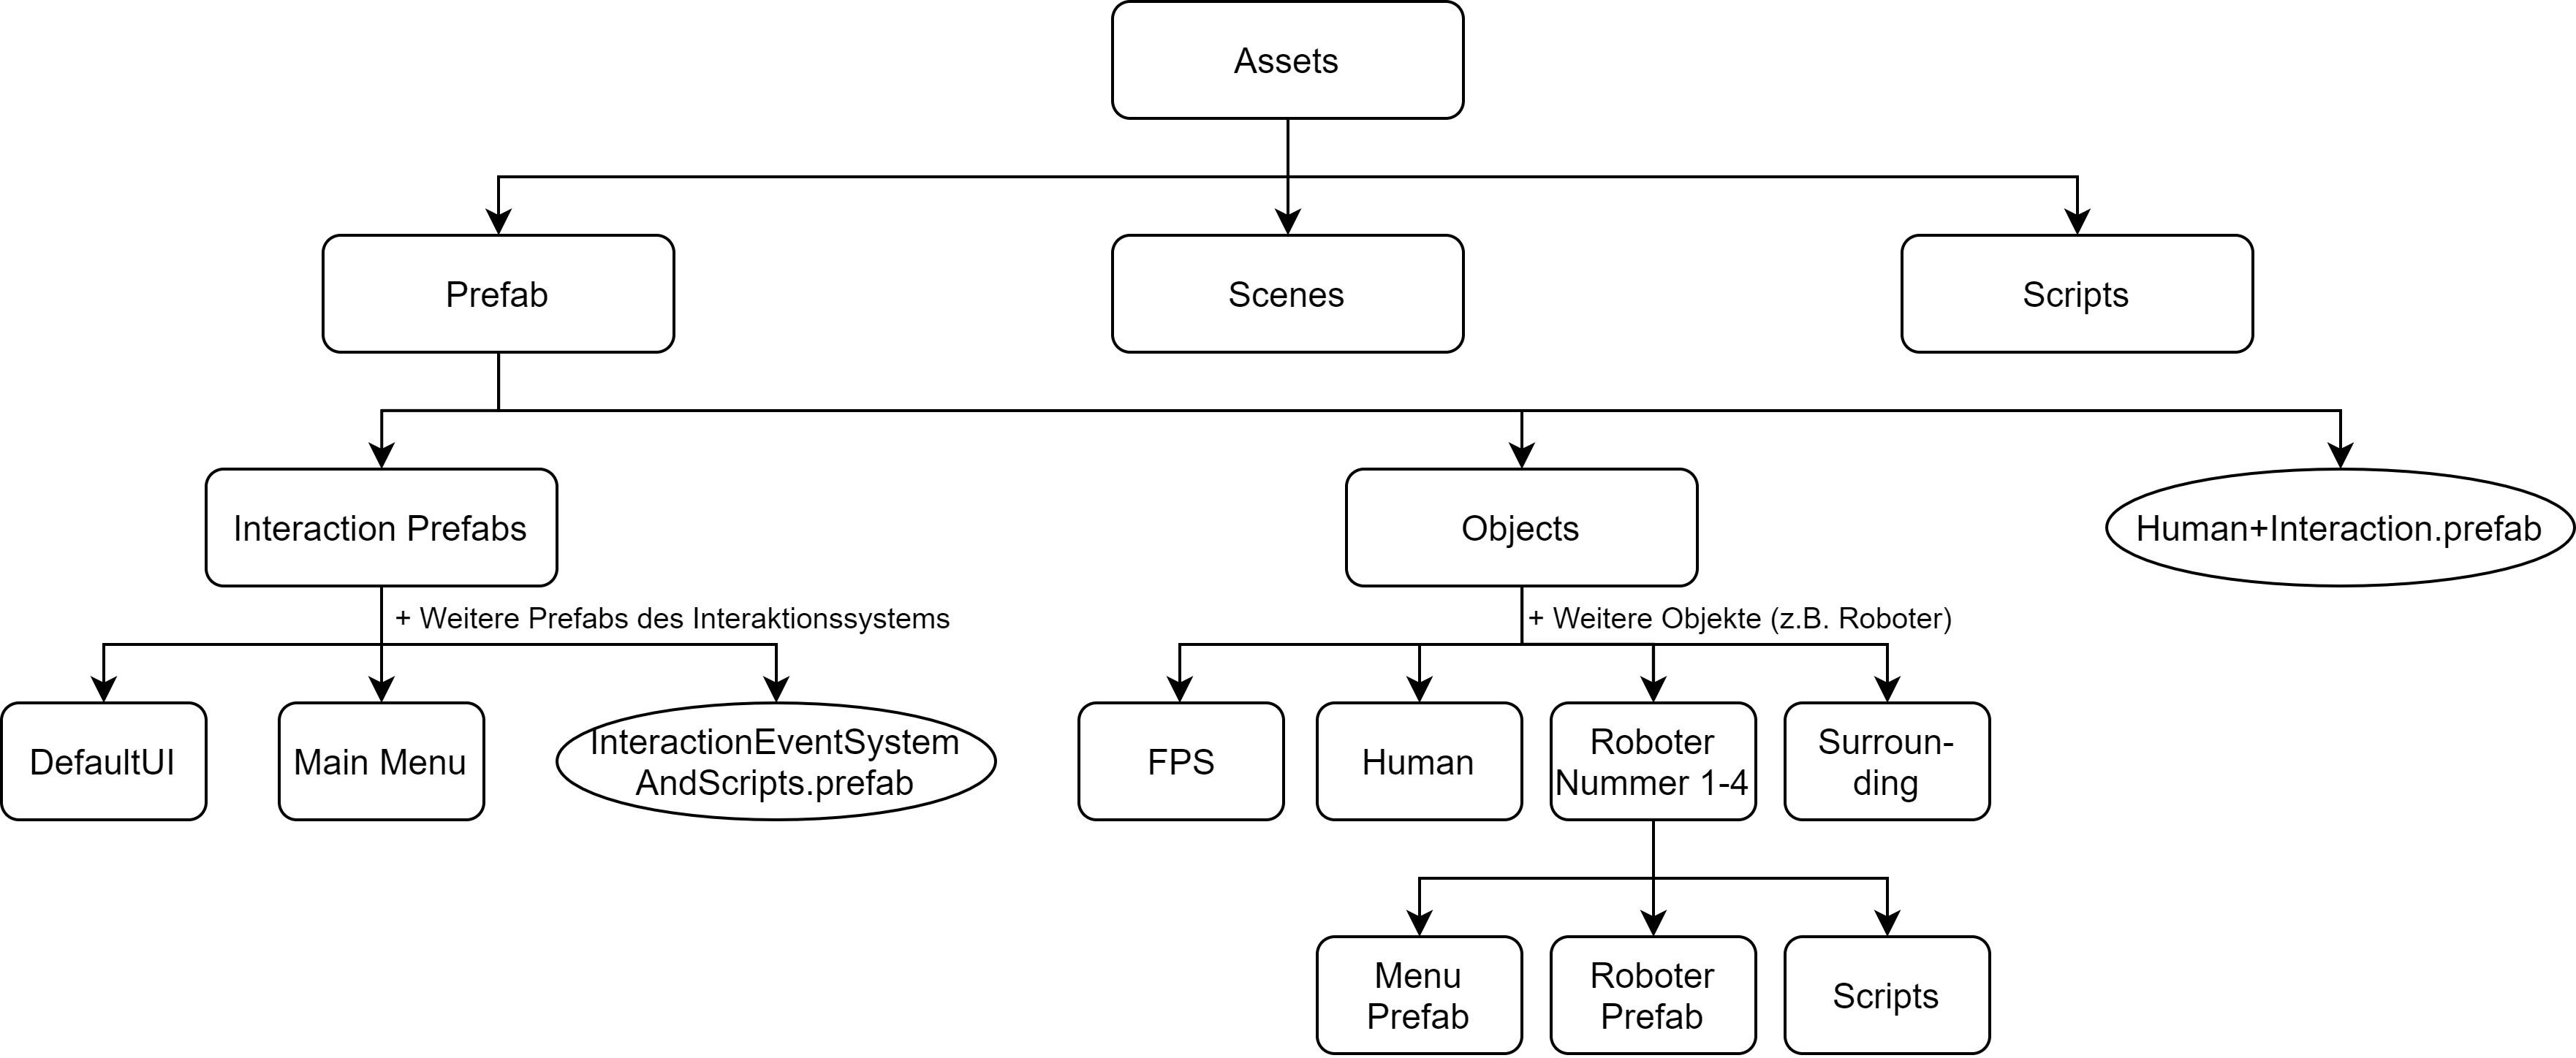
\includegraphics[width=1\linewidth]{Bilder/A54_Ordnerstruktur}
	\caption{Die Ordnerstruktur des Projekts, eigene Abbildung}
	\label{fig:Ordnerstruktur}
\end{figure}
\newline
Auf der obersten Ebene des Projekts befinden sich die Ordner \textbf{'Prefab'}, \textbf{'Scenes'} und \textbf{'Scripts'}. In dem Ordner 'Scenes' befinden sich die drei Demo-Szenen und in dem Ordner 'Scripts' die Skripte abgespeichert. Neben den vorhandenen Demo-Szenen empfiehlt es sich in Zukunft, alle weiteren Szenen des Projekts in diesem Ordner abzuspeichern. Im Gegensatz dazu, sollte der Inhalt des Ordners 'Scripts' größtenteils unverändert bleiben, da sich in diesem Ordner die Skripte für das Menschmodell und die Interaktionsschnittstelle befinden. Lediglich das Skript Global Variables, welches sich in einem eigenen Unterordner befinden, sollte angepasst werden, falls neue Objekte in die Umgebung eingefügt werden. Des Weiteren ist anzumerken, dass sich, neben diesen drei Ordnern, noch weitere Ordner auf dieser Ebene im Projekt befinden. Diese sind aber, wie z.B. in Abbildung \ref{fig:UnityOverview} zu erkennen ist, automatisch generierte Ordner, die durch das Importieren der Plugins Final IK und SteamVR entstehen und daher an dieser Stelle vernachlässigbar. 
\newline\newline
In Abbildungen \ref{fig:Ordnerstruktur} sind nur die Unterordner des Ordners 'Prefab' abgebildet, da der Inhalt der Ordner 'Scenes' und 'Scripts' bereits erläutert wurde. Insgesamt enthält der Ordner 'Prefab', neben dem Prefab des fertigen Menschmodells inklusive der Interaktionsschnittstelle ('Human+Interaction.prefab', vgl. Abbildung \ref{fig:UnityOverview}), noch zwei weitere Unterordner.\newline
Der erste Unterordner trägt den Namen \textbf{'Interaction Prefabs'} und enthält alle Prefabs des Interaktionssystems, u.a. auch das in Abbildung \ref{fig:UnityOverview} dargestellte Objekt 'InteractionEventSystemAndScripts' Prefab. Des Weiteren befinden sich in den Unterordnern DefaultUI und Main Menu ein Beispiel einer graphischen Benutzeroberfläche und das in Kapitel \ref{sec:WeitereTeileInteraktion} dargestellte Hauptmenü, inklusive der zugehörigen Skripte. Der Inhalt des Ordners DefaultUI kann als Vorlage für neue graphische Benutzeroberflächen verwendet werden. Außerdem kann bei Bedarf das Main Menu bearbeitet werden. Durch den modularen Aufbau der Komponenten der Interaktionsschnittstelle, können bei Bedarf die einzelnen Komponenten, wie beispielsweise die Pointer oder das Event System, bearbeitet werden.\newline
Der Zweite Unterordner trägt den Namen \textbf{'Objects'} und enthält alle weiteren Objekte die sich in der Szene befinden. Dabei sollte in der Regel der Inhalt der Ordner 'FPS' und 'Human' nicht verändert werden, es sei denn es sollen Veränderungen am Menschmodell vorgenommen werden. Im Ordner 'FPS' befindet sich lediglich die für Entwicklungszwecke eingesetzte 'Frames per Second' Komponente. Mit Hilfe dieser Komponente lässt sich die aktuelle Bildwiederholrate auslesen. Die in Abbildung \ref{fig:UnityOverview} dargestellten einzelnen Komponenten des eigentlichen Menschmodells, ohne die Interaktionsschnittstelle, befinden sich alle in dem Unterordner 'Human'. Die restlichen Unterordner werden, wie bereits erwähnt, dafür genutzt um alle weiteren Objekte abzuspeichern. Bei dieser Arbeit wurden alle Komponenten der Umgebung (Wände, Böden, etc.) in dem Unterordner 'Surrounding' abgespeichert. Es emfpiehlt sich, für alle Objekte mit denen Interagiert werden soll, wie in Abbildung \ref{fig:Ordnerstruktur} dargestellt, jeweils einen eigenen Unterordner anzulegen. Durch diese Struktur wird deutlich, dass beliebige Objekte hinzugefügt werden können, die in keinster Weise abhängig voneinander, von der Interaktionsschnittstelle oder vom Menschmodell sind. Jedes Objekt kann seine eigene interne Ordnerstruktur besitzen um alle Objektvorlagen, Bilder, Skripte etc. zu organisieren.
	
\paragraph{2. Einsatzfähig für die Interaktionsschnittstelle machen}
\noindent Neue Objekte Einsatzfähig für die Interaktionsschnittstelle zu machen erfordert, dass diese zunächst in der Szene platziert und um das in Kapitel \ref{sec:GrundgerüstInteraktion} erläuterte Skript Object Menu erweitert werden. Dazu kann einfach das Skript per Drag and Drop auf das gewünschte Objekt gezogen werden. Wie in Abbildung \ref{fig:ObjectMenu} zu erkennen ist, müssen in dem Skript noch ein paar Anpassungen gemacht werden. Zunächst müssen, ebenfalls per Drag and Drop, Referenzen auf die Objektvorlage des eigentlichen Objekts (thisObject) und des zugehörigen Menüs (prefab) gemacht werden. Daraufhin kann über die Auswahllisten bei Click Button und Click Action die gewünschte Taste am rechten oder linken Controller, mit der das Menü wieder geschlossen werden kann, ausgewählt werden. Es ist anzumerken, dass wie bereits in Kapitel \ref{sec:GrundgerüstInteraktion} erwähnt, das Objekt über einen Collider verfügen muss. Diese Anforderung wird erfüllt, indem einfach über den Knopf 'Add Component' im Inspektor ein Box Collider zu dem Objekt hinzugefügt wird. Dieser Box-Collider muss jedoch an die Größe des Objekts angepasst werden, um eine Präzise Interaktion zu ermöglichen. Des Weiteren kann auf Wunsch das in Kapitel \ref{sec:WeitereTeileInteraktion} erläuterte Skript PointerEvent\_Objects zu dem Objekt hinzugefügt werden, um dem Bediener bei der Interaktion ein visuelles Feedback zu geben. Sobald alle diese Schritte abgeschlossen sind, ist das gewünschte Objekt einsatzfähig für die Interaktionsschnittstelle gemacht worden. Im letzten Schritt sollte das Objekt aus der Hierarchie-Ansicht per Drag and Drop in den dazugehörigen Ordner gezogen werden, um es als neues Prefab mit den angesprochenen Erweiterungen zu speichern, sodass es später bei Bedarf beliebig oft instanziiert werden kann.

\paragraph{3. Einbinden in das vorhandene Menü (Optional)}
\noindent Bevor der letzte Schritt der Vorgehensweise beim hinzufügen neuer Objekte in der Umgebung erläutert wird, ist anzumerken, dass dieser Schritt nur optional ist, da die im folgenden Behandelten Komponenten, wie bereits in Kapitel \ref{sec:WeitereTeileInteraktion} erwähnt, nur zu Demonstrationszwecken und um ein Anwendungsbeispiel für die Interaktionsschnittstelle zu schaffen, hinzugefügt wurden. Zunächst müsste das Inventar des Hauptmenüs (Vgl. Abbildung \ref{fig:MainMenu}) angepasst und um entsprechende Knöpfe für das instanziieren des gewünschten Objekts erweitert werden. Dazu müssten auch die zugehörigen Skripte des Menüs aus dem Ordner 'Main Menu' angepasst werden (Vgl. Abbildung \ref{fig:Ordnerstruktur}). Des Weiteren müsste das Skripte Global Variables angepasst werden. Konkret bedeutet dass, dass das hinzugefügte Objekt im Skript Global Variables vermerkt werden muss. Dazu muss zunächst in einer öffentlichen Variable vom Typ GameObject eine Referenz zum Prefab des Objekts gesetzt werden, damit dieses beispielsweise von dem Skript Spawning Handler aufgerufen werden kann. Des Weiteren muss in öffentlichen Variablen vom Typ Integer das maximale und initiale Vorkommen des Objekts in der Szene deklariert werden. Schließlich müssen die Arrays, welche die angesprochenen Informationen von allen Objekten, mit denen interagiert werden kann, speichern, um eins verlängert werden. Dieser Prozess könnte in Zukunft einfacher gestaltet werden, indem beispielsweise eine Anbindung an eine Datenbank geschaffen wird, aus der alle Objektvorlagen automatisch geladen und entsprechende Anpassungen in dem Skript Global Variables und im Menü gemacht werden.

%--------------------------------------------------------------------------------------------------
\section{Validierung der Anforderungen des Menschmodells}\label{sec:ValidMensch}

\paragraph{1. Genauigkeit}
\noindent Durch die Möglichkeit, die Bewegungen des Bedieners an bis zu zehn Körperteilen (Beide Füße, beide Knie, Steißbein, beide Hände, beide Ellenbogen und Kopf) zu verfolgen und diese Daten bei der Abbildung auf den virtuellen Menschen zu berücksichtigen, wird die in Kapitel \ref{sec:AnforderungenKonzept} geforderte Genauigkeit erfüllt. Zusätzlich wird die Genauigkeit, durch die Möglichkeit das Menschmodell zu Kalibrieren, also an die Körpergröße des Bedieners anzupassen, verbessert. So könnte in Zukunft für jeden beliebigen Bediener, mit Hilfe des Menschmodells, ein virtueller Klon für die virtuelle Welt geschaffen werden, in dem die Textur für den in Kapitel \ref{sec:MMModell} angesprochenen Skinned Mesh Renderer, angepasst wird.
	
\paragraph{2. Echtzeit}
\noindent Mit Hilfe des Plugins Final IK werden die Bewegungsdaten des Bedieners in nahezu Echtzeit verarbeitet und auf das Menschmodell übertragen. Es sind keine sichtbaren Verzögerungen zu erkennen, die die Nützlichkeit des Menschmodells einschränken würden oder sogar eine potenzielle Gefahrenquelle darstellen könnten. Aufgrund dessen wird die in Kapitel \ref{sec:AnforderungenKonzept} gestellte Anforderung an die Echtzeit ebenfalls erfüllt.
	
\paragraph{3. Interoperabilität}
\noindent Das Menschmodell wurde umgebungsunabhängig implementiert, ist also von keinen anderen Komponenten der virtuellen Umgebung abhängig. Folglich kann das Menschmodell in jeder beliebigen virtuellen Umgebung, wie beispielsweise in einer virtuell begehbaren Produktionsanlagen, eingesetzt werden und erfüllt somit die in Kapitel \ref{sec:AnforderungenKonzept} gestellte Anforderung an die Interoperabilität.
	
\paragraph{4. Modularität}
\noindent Wie in Abbildung \ref{fig:UnityOverview} zu erkennen ist, ist das Menschmodell modular aufgebaut und erlaubt einfache Anpassungen und Erweiterungen in der Zukunft. Insgesamt besteht das Menschmodell (ohne die Interaktionsschnittstelle) aus den vier Komponenten: Kamera, Modell, Skripte und Verfolgungsziele. Diese bestehen teilweise selber nochmal aus einigen Komponenten. Aufgrund dessen wird die in Kapitel \ref{sec:AnforderungenKonzept} geforderte Modularität gewährleistet.

%--------------------------------------------------------------------------------------------------
\section{Validierung der Anforderungen der Interaktionsschnittstelle}\label{sec:ValidInteraktion}

\paragraph{1. Bidirektionalität}
\noindent Der Informationsaustausch zwischen Mensch und Maschine findet bidirektional statt, da der Mensch durch den Pointer die Möglichkeit erhält über graphische Benutzeroberflächen mit der Maschine zu interagieren. In anderen Worten stellt der Pointer das Input-Medium des Menschen dar. Gleichzeitig ermöglichen die graphischen Benutzeroberflächen die Darstellung von Feedback der Produktionsanlagen. So könnten beispielsweise Produktionsraten, Stromverbrauch oder sonstige produktionstechnisch relevante Parameter angezeigt werden. Aufgrund dessen wird die in Kapitel \ref{sec:AnforderungenKonzept} geforderte Anforderung der Bidirektionalität erfüllt.
	
\paragraph{2. Genauigkeit}
\noindent Mit Hilfe des Pointers, der durch das Bewegen der rechten Hand gesteuert wird, wird ein sehr präzises und vor allem intuitives interagieren mit der Umgebung ermöglicht. Aufgrund dessen wird die in Kapitel \ref{sec:AnforderungenKonzept} geforderte Genauigkeit bei der Interaktion mit der Umgebung gewährleistet.
	
\paragraph{3. Echtzeit}
\noindent Durch die Verarbeitung der Bewegungsdaten in Echtzeit wird nicht nur die nahezu verzögerungslose Abbildung des Menschmodells, sondern auch eine nahezu verzögerungslose Interaktion mit der Umgebung ermöglicht. Dies ermöglicht den Bedienern schnell auf Veränderungen in der virtuellen Umgebung zu reagieren und spontane Anpassungen zu tätigen. Aufgrund dessen wird die in Kapitel \ref{sec:AnforderungenKonzept} gestellte Anforderung an die Echtzeit ebenfalls erfüllt.
	
\paragraph{4. Interoperabilität}
\noindent Die Interaktionsschnittstelle ist, bis auf wenige Skripte und dem Interaktionssystem, nicht von der Umgebung abhängig. Daher ist es ausreichend, diese Komponenten irgendwo in der Szene zu hinterlegen (Vgl. Abbildung \ref{fig:UnityOverview}). Eine Interaktion mit beliebigen Objekten in der Szene zu ermöglichen erfordert, dass diese lediglich das Object Menu Skript und einem Collider erhalten. Des Weiteren müssen ihre Menüs mit Hilfe der bereits in Unity vorhanden Komponenten für graphische Benutzeroberflächen implementiert sein. Folglich wird die in Kapitel \ref{sec:AnforderungenKonzept} geforderte Interoperabilität gewährleistet, da sich die beschrieben Funktionalität auf beliebige Objekte übertragen lässt, solange die entsprechenden Rahmenbedingungen eingehalten werden.
	
\paragraph{5. Modularität}
\noindent Sowohl das Menschmodell, als auch die Interaktionsschnittstelle, sind Modular aufgebaut und bestehe aus austauschbaren Komponenten. Es ist beispielsweise möglich, die Interaktionsschnittstelle für andere VR Hardware einsatzfähig zu machen. Dafür müssen lediglich die entsprechenden Input Schnittstellen der VR Hardware in einigen Skripten angepasst werden. Des Weiteren wurden das Menschmodell und die Interaktionsschnittstelle getrennt voneinander entwickelt, um die Unabhängigkeit und somit die in Kapitel \ref{sec:AnforderungenKonzept} geforderte Modularität zu gewährleisten.

%--------------------------------------------------------------------------------------------------